% Generated by make_fig_b_tool.py from teleport_chain.py, srcML and the tool. Do not edit by hand.
\documentclass[tikz,border=2pt]{standalone}
\usepackage[T1]{fontenc}
\usepackage{newtxtext,newtxmath}
\usepackage[varqu,scaled=0.95]{zi4}
\usetikzlibrary{arrows.meta,calc,backgrounds}
\definecolor{ink}{HTML}{1F2328}\definecolor{mute}{HTML}{6E7781}\definecolor{rule}{HTML}{D0D7DE}
\definecolor{tagC}{HTML}{8C959F}\definecolor{srcbg}{HTML}{F3F5F7}\definecolor{wire}{HTML}{24527F}
\definecolor{gateC}{HTML}{24527F}\definecolor{gateL}{HTML}{DCE7F3}
\definecolor{qubC}{HTML}{1A7F64}\definecolor{qubL}{HTML}{D8F0E8}
\definecolor{bitC}{HTML}{A64B00}\definecolor{bitL}{HTML}{FBE7D3}
\definecolor{condC}{HTML}{6639BA}\definecolor{condL}{HTML}{ECE4F8}
\definecolor{posC}{HTML}{1F2328}\definecolor{posL}{HTML}{E1E5E9}
\newcommand{\role}[3]{{\setlength{\fboxsep}{0.6pt}\colorbox{#2}{\strut\textcolor{#1}{\bfseries #3}}}}
\tikzset{
  >={Stealth[length=3.6pt,width=3.2pt]},
  stage/.style={font=\fontsize{9}{11}\selectfont\bfseries, text=ink, anchor=west, inner sep=0pt},
  stnum/.style={circle, draw=ink, line width=0.6pt, font=\fontsize{8}{9}\selectfont\bfseries, text=ink, inner sep=0pt, minimum size=11pt},
  xml/.style={font=\ttfamily\fontsize{9}{11}\selectfont, anchor=west, inner sep=0pt},
  pyline/.style={font=\ttfamily\fontsize{9}{11}\selectfont, anchor=west, inner sep=0pt, text=ink},
  lab/.style={font=\fontsize{8.5}{10}\selectfont, anchor=west, inner sep=0pt, text=mute},
  flowarrow/.style={->, line width=0.7pt, draw=ink},
}
\begin{document}
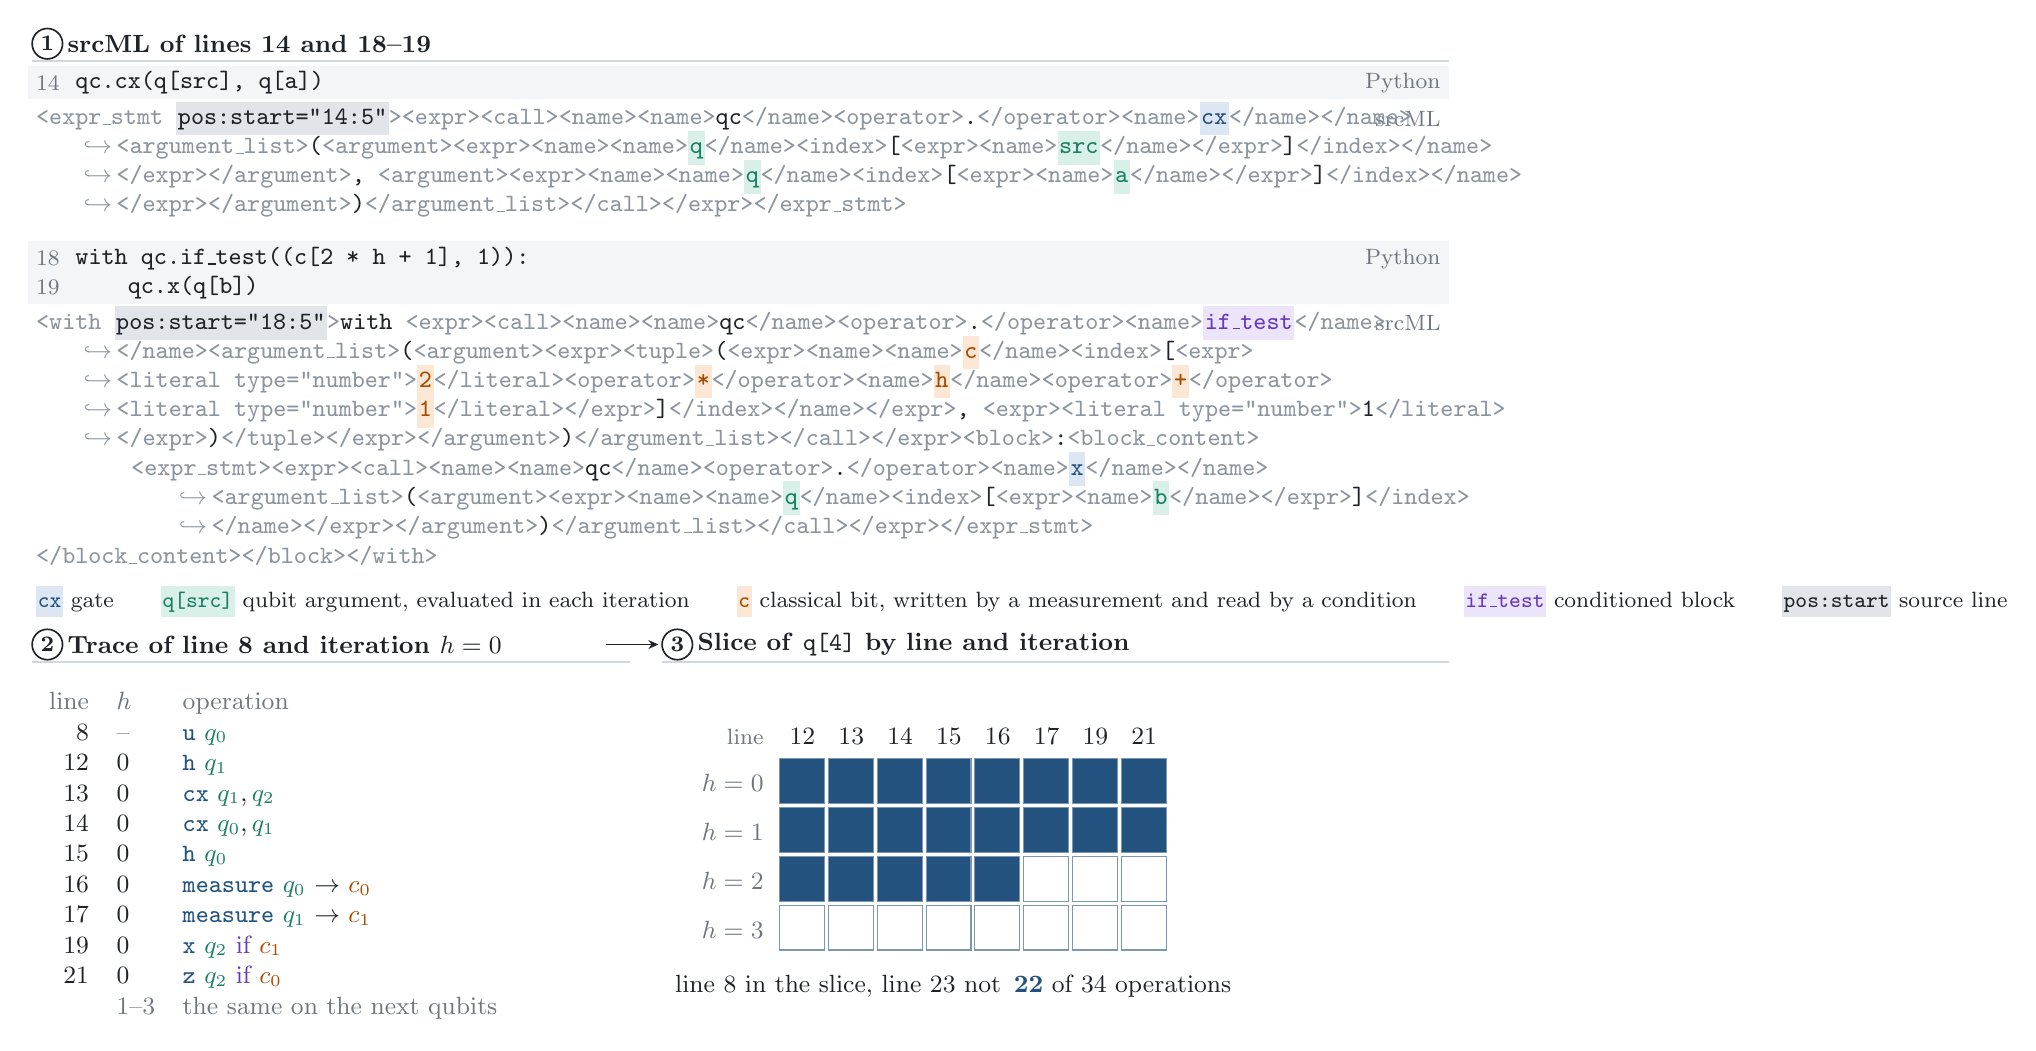
\begin{tikzpicture}

\node[stnum] at (0.2,0.5) {1};
\node[stage] at (0.45,0.5) {srcML of lines 14 and 18--19};
\draw[rule, line width=0.6pt] (0,0.28) -- (18.0,0.28);
\node[lab] at (0.05,0.000) {14};
\node[pyline] at (0.55,0.000) {qc.cx(q[src],\ q[a])};
\begin{scope}[on background layer]\fill[srcbg] (-0.05,0.220) rectangle (18.0,-0.200);\end{scope}
\node[lab, anchor=east] at (17.9,0.000) {Python};
\node[lab, anchor=east] at (17.9,-0.450) {srcML};
\node[xml] at (0.05,-0.450) {\textcolor{tagC}{<expr\_stmt }\role{posC}{posL}{pos:start="14:5"}\textcolor{tagC}{>}\textcolor{tagC}{<expr>}\textcolor{tagC}{<call>}\textcolor{tagC}{<name>}\textcolor{tagC}{<name>}\textcolor{ink}{qc}\textcolor{tagC}{</name>}\textcolor{tagC}{<operator>}\textcolor{ink}{.}\textcolor{tagC}{</operator>}\textcolor{tagC}{<name>}\role{gateC}{gateL}{cx}\textcolor{tagC}{</name>}\textcolor{tagC}{</name>}};
\node[xml] at (0.654,-0.820) {\textcolor{tagC}{\rmfamily\fontsize{9}{11}\selectfont$\hookrightarrow$}\,\textcolor{tagC}{<argument\_list>}\textcolor{ink}{(}\textcolor{tagC}{<argument>}\textcolor{tagC}{<expr>}\textcolor{tagC}{<name>}\textcolor{tagC}{<name>}\role{qubC}{qubL}{q}\textcolor{tagC}{</name>}\textcolor{tagC}{<index>}\textcolor{ink}{[}\textcolor{tagC}{<expr>}\textcolor{tagC}{<name>}\role{qubC}{qubL}{src}\textcolor{tagC}{</name>}\textcolor{tagC}{</expr>}\textcolor{ink}{]}\textcolor{tagC}{</index>}\textcolor{tagC}{</name>}};
\node[xml] at (0.654,-1.190) {\textcolor{tagC}{\rmfamily\fontsize{9}{11}\selectfont$\hookrightarrow$}\,\textcolor{tagC}{</expr>}\textcolor{tagC}{</argument>}\textcolor{ink}{, }\textcolor{tagC}{<argument>}\textcolor{tagC}{<expr>}\textcolor{tagC}{<name>}\textcolor{tagC}{<name>}\role{qubC}{qubL}{q}\textcolor{tagC}{</name>}\textcolor{tagC}{<index>}\textcolor{ink}{[}\textcolor{tagC}{<expr>}\textcolor{tagC}{<name>}\role{qubC}{qubL}{a}\textcolor{tagC}{</name>}\textcolor{tagC}{</expr>}\textcolor{ink}{]}\textcolor{tagC}{</index>}\textcolor{tagC}{</name>}};
\node[xml] at (0.654,-1.560) {\textcolor{tagC}{\rmfamily\fontsize{9}{11}\selectfont$\hookrightarrow$}\,\textcolor{tagC}{</expr>}\textcolor{tagC}{</argument>}\textcolor{ink}{)}\textcolor{tagC}{</argument\_list>}\textcolor{tagC}{</call>}\textcolor{tagC}{</expr>}\textcolor{tagC}{</expr\_stmt>}};
\node[lab] at (0.05,-2.230) {18};
\node[pyline] at (0.55,-2.230) {with\ qc.if\_test((c[2\ *\ h\ +\ 1],\ 1)):};
\node[lab] at (0.05,-2.600) {19};
\node[pyline] at (0.55,-2.600) {\ \ \ \ qc.x(q[b])};
\begin{scope}[on background layer]\fill[srcbg] (-0.05,-2.010) rectangle (18.0,-2.800);\end{scope}
\node[lab, anchor=east] at (17.9,-2.230) {Python};
\node[lab, anchor=east] at (17.9,-3.050) {srcML};
\node[xml] at (0.05,-3.050) {\textcolor{tagC}{<with }\role{posC}{posL}{pos:start="18:5"}\textcolor{tagC}{>}\textcolor{ink}{with }\textcolor{tagC}{<expr>}\textcolor{tagC}{<call>}\textcolor{tagC}{<name>}\textcolor{tagC}{<name>}\textcolor{ink}{qc}\textcolor{tagC}{</name>}\textcolor{tagC}{<operator>}\textcolor{ink}{.}\textcolor{tagC}{</operator>}\textcolor{tagC}{<name>}\role{condC}{condL}{if\_test}\textcolor{tagC}{</name>}};
\node[xml] at (0.654,-3.420) {\textcolor{tagC}{\rmfamily\fontsize{9}{11}\selectfont$\hookrightarrow$}\,\textcolor{tagC}{</name>}\textcolor{tagC}{<argument\_list>}\textcolor{ink}{(}\textcolor{tagC}{<argument>}\textcolor{tagC}{<expr>}\textcolor{tagC}{<tuple>}\textcolor{ink}{(}\textcolor{tagC}{<expr>}\textcolor{tagC}{<name>}\textcolor{tagC}{<name>}\role{bitC}{bitL}{c}\textcolor{tagC}{</name>}\textcolor{tagC}{<index>}\textcolor{ink}{[}\textcolor{tagC}{<expr>}};
\node[xml] at (0.654,-3.790) {\textcolor{tagC}{\rmfamily\fontsize{9}{11}\selectfont$\hookrightarrow$}\,\textcolor{tagC}{<literal type="number">}\role{bitC}{bitL}{2}\textcolor{tagC}{</literal>}\textcolor{ink}{ }\textcolor{tagC}{<operator>}\role{bitC}{bitL}{*}\textcolor{tagC}{</operator>}\textcolor{ink}{ }\textcolor{tagC}{<name>}\role{bitC}{bitL}{h}\textcolor{tagC}{</name>}\textcolor{ink}{ }\textcolor{tagC}{<operator>}\role{bitC}{bitL}{+}\textcolor{tagC}{</operator>}\textcolor{ink}{ }};
\node[xml] at (0.654,-4.160) {\textcolor{tagC}{\rmfamily\fontsize{9}{11}\selectfont$\hookrightarrow$}\,\textcolor{tagC}{<literal type="number">}\role{bitC}{bitL}{1}\textcolor{tagC}{</literal>}\textcolor{tagC}{</expr>}\textcolor{ink}{]}\textcolor{tagC}{</index>}\textcolor{tagC}{</name>}\textcolor{tagC}{</expr>}\textcolor{ink}{, }\textcolor{tagC}{<expr>}\textcolor{tagC}{<literal type="number">}\textcolor{ink}{1}\textcolor{tagC}{</literal>}};
\node[xml] at (0.654,-4.530) {\textcolor{tagC}{\rmfamily\fontsize{9}{11}\selectfont$\hookrightarrow$}\,\textcolor{tagC}{</expr>}\textcolor{ink}{)}\textcolor{tagC}{</tuple>}\textcolor{tagC}{</expr>}\textcolor{tagC}{</argument>}\textcolor{ink}{)}\textcolor{tagC}{</argument\_list>}\textcolor{tagC}{</call>}\textcolor{tagC}{</expr>}\textcolor{tagC}{<block>}\textcolor{ink}{:}\textcolor{tagC}{<block\_content>}};
\node[xml] at (1.258,-4.900) {\textcolor{tagC}{<expr\_stmt>}\textcolor{tagC}{<expr>}\textcolor{tagC}{<call>}\textcolor{tagC}{<name>}\textcolor{tagC}{<name>}\textcolor{ink}{qc}\textcolor{tagC}{</name>}\textcolor{tagC}{<operator>}\textcolor{ink}{.}\textcolor{tagC}{</operator>}\textcolor{tagC}{<name>}\role{gateC}{gateL}{x}\textcolor{tagC}{</name>}\textcolor{tagC}{</name>}};
\node[xml] at (1.8619999999999999,-5.270) {\textcolor{tagC}{\rmfamily\fontsize{9}{11}\selectfont$\hookrightarrow$}\,\textcolor{tagC}{<argument\_list>}\textcolor{ink}{(}\textcolor{tagC}{<argument>}\textcolor{tagC}{<expr>}\textcolor{tagC}{<name>}\textcolor{tagC}{<name>}\role{qubC}{qubL}{q}\textcolor{tagC}{</name>}\textcolor{tagC}{<index>}\textcolor{ink}{[}\textcolor{tagC}{<expr>}\textcolor{tagC}{<name>}\role{qubC}{qubL}{b}\textcolor{tagC}{</name>}\textcolor{tagC}{</expr>}\textcolor{ink}{]}\textcolor{tagC}{</index>}};
\node[xml] at (1.8619999999999999,-5.640) {\textcolor{tagC}{\rmfamily\fontsize{9}{11}\selectfont$\hookrightarrow$}\,\textcolor{tagC}{</name>}\textcolor{tagC}{</expr>}\textcolor{tagC}{</argument>}\textcolor{ink}{)}\textcolor{tagC}{</argument\_list>}\textcolor{tagC}{</call>}\textcolor{tagC}{</expr>}\textcolor{tagC}{</expr\_stmt>}};
\node[xml] at (0.05,-6.010) {\textcolor{tagC}{</block\_content>}\textcolor{tagC}{</block>}\textcolor{tagC}{</with>}};
\node[anchor=north west, font=\fontsize{8.5}{10}\selectfont, inner sep=0pt] at (0.05,-6.380) {{\ttfamily \role{gateC}{gateL}{cx}}\ \textcolor{ink}{gate}\qquad {\ttfamily \role{qubC}{qubL}{q[src]}}\ \textcolor{ink}{qubit argument, evaluated in each iteration}\qquad {\ttfamily \role{bitC}{bitL}{c}}\ \textcolor{ink}{classical bit, written by a measurement and read by a condition}\qquad {\ttfamily \role{condC}{condL}{if\_test}}\ \textcolor{ink}{conditioned block}\qquad {\ttfamily \role{posC}{posL}{pos:start}}\ \textcolor{ink}{source line}};
\begin{scope}[yshift=-7.630cm]
\node[stnum] at (0.2,0.5) {2};
\node[stage] at (0.45,0.5) {Trace of line 8 and iteration $h = 0$};
\draw[rule, line width=0.6pt] (0.0,0.28) -- (7.6,0.28);
\node[anchor=north west, font=\fontsize{9}{11}\selectfont, text=ink, inner sep=0pt] at (0.04,-0.05) {\setlength{\tabcolsep}{5pt}\begin{tabular}{rll}\textcolor{mute}{line}&\textcolor{mute}{$h$}&\textcolor{mute}{operation}\\[0pt]8&\textcolor{mute}{--}&\textcolor{gateC}{\texttt{u}} \textcolor{qubC}{$q_{0}$}\\[0pt]12&0&\textcolor{gateC}{\texttt{h}} \textcolor{qubC}{$q_{1}$}\\[0pt]13&0&\textcolor{gateC}{\texttt{cx}} \textcolor{qubC}{$q_{1}$},\,\textcolor{qubC}{$q_{2}$}\\[0pt]14&0&\textcolor{gateC}{\texttt{cx}} \textcolor{qubC}{$q_{0}$},\,\textcolor{qubC}{$q_{1}$}\\[0pt]15&0&\textcolor{gateC}{\texttt{h}} \textcolor{qubC}{$q_{0}$}\\[0pt]16&0&\textcolor{gateC}{\texttt{measure}} \textcolor{qubC}{$q_{0}$} $\to$ \textcolor{bitC}{$c_{0}$}\\[0pt]17&0&\textcolor{gateC}{\texttt{measure}} \textcolor{qubC}{$q_{1}$} $\to$ \textcolor{bitC}{$c_{1}$}\\[0pt]19&0&\textcolor{gateC}{\texttt{x}} \textcolor{qubC}{$q_{2}$} \textcolor{condC}{if} \textcolor{bitC}{$c_{1}$}\\[0pt]21&0&\textcolor{gateC}{\texttt{z}} \textcolor{qubC}{$q_{2}$} \textcolor{condC}{if} \textcolor{bitC}{$c_{0}$}\\[0pt]&\textcolor{mute}{1--3}&\textcolor{mute}{the same on the next qubits}\\[0pt]\end{tabular}};
\node[stnum] at (8.2,0.5) {3};
\node[stage] at (8.45,0.5) {Slice of \texttt{q[4]} by line and iteration};
\draw[rule, line width=0.6pt] (8.0,0.28) -- (18.0,0.28);
\node[font=\fontsize{8.5}{10}\selectfont, text=mute, anchor=south east] at (9.42,-0.8999999999999999) {line};
\node[font=\fontsize{9}{11}\selectfont, text=ink, anchor=south] at (9.790000000000001,-0.8999999999999999) {12};
\node[font=\fontsize{9}{11}\selectfont, text=ink, anchor=south] at (10.41,-0.8999999999999999) {13};
\node[font=\fontsize{9}{11}\selectfont, text=ink, anchor=south] at (11.030000000000001,-0.8999999999999999) {14};
\node[font=\fontsize{9}{11}\selectfont, text=ink, anchor=south] at (11.65,-0.8999999999999999) {15};
\node[font=\fontsize{9}{11}\selectfont, text=ink, anchor=south] at (12.270000000000001,-0.8999999999999999) {16};
\node[font=\fontsize{9}{11}\selectfont, text=ink, anchor=south] at (12.89,-0.8999999999999999) {17};
\node[font=\fontsize{9}{11}\selectfont, text=ink, anchor=south] at (13.51,-0.8999999999999999) {19};
\node[font=\fontsize{9}{11}\selectfont, text=ink, anchor=south] at (14.13,-0.8999999999999999) {21};
\node[font=\fontsize{9}{11}\selectfont, text=mute, anchor=east] at (9.42,-1.26) {$h = 0$};
\draw[draw=wire!60, line width=0.4pt, fill=wire] (9.5,-0.95) rectangle ++(0.57,-0.57);
\draw[draw=wire!60, line width=0.4pt, fill=wire] (10.12,-0.95) rectangle ++(0.57,-0.57);
\draw[draw=wire!60, line width=0.4pt, fill=wire] (10.74,-0.95) rectangle ++(0.57,-0.57);
\draw[draw=wire!60, line width=0.4pt, fill=wire] (11.36,-0.95) rectangle ++(0.57,-0.57);
\draw[draw=wire!60, line width=0.4pt, fill=wire] (11.98,-0.95) rectangle ++(0.57,-0.57);
\draw[draw=wire!60, line width=0.4pt, fill=wire] (12.6,-0.95) rectangle ++(0.57,-0.57);
\draw[draw=wire!60, line width=0.4pt, fill=wire] (13.219999999999999,-0.95) rectangle ++(0.57,-0.57);
\draw[draw=wire!60, line width=0.4pt, fill=wire] (13.84,-0.95) rectangle ++(0.57,-0.57);
\node[font=\fontsize{9}{11}\selectfont, text=mute, anchor=east] at (9.42,-1.88) {$h = 1$};
\draw[draw=wire!60, line width=0.4pt, fill=wire] (9.5,-1.5699999999999998) rectangle ++(0.57,-0.57);
\draw[draw=wire!60, line width=0.4pt, fill=wire] (10.12,-1.5699999999999998) rectangle ++(0.57,-0.57);
\draw[draw=wire!60, line width=0.4pt, fill=wire] (10.74,-1.5699999999999998) rectangle ++(0.57,-0.57);
\draw[draw=wire!60, line width=0.4pt, fill=wire] (11.36,-1.5699999999999998) rectangle ++(0.57,-0.57);
\draw[draw=wire!60, line width=0.4pt, fill=wire] (11.98,-1.5699999999999998) rectangle ++(0.57,-0.57);
\draw[draw=wire!60, line width=0.4pt, fill=wire] (12.6,-1.5699999999999998) rectangle ++(0.57,-0.57);
\draw[draw=wire!60, line width=0.4pt, fill=wire] (13.219999999999999,-1.5699999999999998) rectangle ++(0.57,-0.57);
\draw[draw=wire!60, line width=0.4pt, fill=wire] (13.84,-1.5699999999999998) rectangle ++(0.57,-0.57);
\node[font=\fontsize{9}{11}\selectfont, text=mute, anchor=east] at (9.42,-2.5) {$h = 2$};
\draw[draw=wire!60, line width=0.4pt, fill=wire] (9.5,-2.19) rectangle ++(0.57,-0.57);
\draw[draw=wire!60, line width=0.4pt, fill=wire] (10.12,-2.19) rectangle ++(0.57,-0.57);
\draw[draw=wire!60, line width=0.4pt, fill=wire] (10.74,-2.19) rectangle ++(0.57,-0.57);
\draw[draw=wire!60, line width=0.4pt, fill=wire] (11.36,-2.19) rectangle ++(0.57,-0.57);
\draw[draw=wire!60, line width=0.4pt, fill=wire] (11.98,-2.19) rectangle ++(0.57,-0.57);
\draw[draw=wire!60, line width=0.4pt, fill=white] (12.6,-2.19) rectangle ++(0.57,-0.57);
\draw[draw=wire!60, line width=0.4pt, fill=white] (13.219999999999999,-2.19) rectangle ++(0.57,-0.57);
\draw[draw=wire!60, line width=0.4pt, fill=white] (13.84,-2.19) rectangle ++(0.57,-0.57);
\node[font=\fontsize{9}{11}\selectfont, text=mute, anchor=east] at (9.42,-3.1199999999999997) {$h = 3$};
\draw[draw=wire!60, line width=0.4pt, fill=white] (9.5,-2.8099999999999996) rectangle ++(0.57,-0.57);
\draw[draw=wire!60, line width=0.4pt, fill=white] (10.12,-2.8099999999999996) rectangle ++(0.57,-0.57);
\draw[draw=wire!60, line width=0.4pt, fill=white] (10.74,-2.8099999999999996) rectangle ++(0.57,-0.57);
\draw[draw=wire!60, line width=0.4pt, fill=white] (11.36,-2.8099999999999996) rectangle ++(0.57,-0.57);
\draw[draw=wire!60, line width=0.4pt, fill=white] (11.98,-2.8099999999999996) rectangle ++(0.57,-0.57);
\draw[draw=wire!60, line width=0.4pt, fill=white] (12.6,-2.8099999999999996) rectangle ++(0.57,-0.57);
\draw[draw=wire!60, line width=0.4pt, fill=white] (13.219999999999999,-2.8099999999999996) rectangle ++(0.57,-0.57);
\draw[draw=wire!60, line width=0.4pt, fill=white] (13.84,-2.8099999999999996) rectangle ++(0.57,-0.57);
\node[font=\fontsize{9}{11}\selectfont, text=ink, anchor=north west, align=left] at (8.05,-3.5799999999999996) {line 8 in the slice, line 23 not\enspace\textcolor{wire}{\bfseries 22} of 34 operations};
\draw[flowarrow] (7.3,0.5) -- (7.96,0.5);
\end{scope}
\end{tikzpicture}
\end{document}
